\documentclass[12pt]{article}
\usepackage[english]{babel}
\usepackage[square,numbers]{natbib}
\bibliographystyle{abbrvnat}
\usepackage{url}
\usepackage[utf8x]{inputenc}
\usepackage{amsmath}
\usepackage{graphicx}
\usepackage{booktabs}
\graphicspath{{images/}}
\usepackage{parskip}
\usepackage{fancyhdr}
\usepackage{vmargin}

\usepackage{tabularx}

\setmarginsrb{3 cm}{2.5 cm}{3 cm}{2.5 cm}{1 cm}{1.5 cm}{1 cm}{1.5 cm}

\title{Investigating Properties of Houses from a New York Airbnb Dataset}                             % Title
\author{Edward Yidong FANG}                               % Author
\date{\today}                                           % Date

\makeatletter
\let\thetitle\@title
\let\theauthor\@author
\let\thedate\@date
\makeatother

\pagestyle{fancy}
\fancyhf{}
\rhead{\theauthor}
\lhead{Intelligent Data Analysis}
\cfoot{\thepage}

\begin{document}

%%%%%%%%%%%%%%%%%%%%%%%%%%%%%%%%%%%%%%%%%%%%%%%%%%%%%%%%%%%%%%%%%%%%%%%%%%%%%%%%%%%%%%%%%

\begin{titlepage}
    \centering
    \vspace*{0.5 cm}
    
\includegraphics[width=0.3\textwidth, trim = {0 90px 0 0}, clip]{images/sustclogo.png}\\[0.0 cm]   % University Logo
    \textsc{\Large Southern University of Science and Technology}\\[2.0 cm]  
    \textsc{\Large CS212 Intelligent Data Analysis}\\[0.5 cm]               
    \large Director: Prof. Peter Ti\v{n}o\\[0.5 cm]             
    \rule{\linewidth}{0.2 mm} \\[0.4 cm]
    { \huge \bfseries \thetitle}\\
    \rule{\linewidth}{0.2 mm} \\[1.5 cm]
    
    \begin{minipage}{0.4\textwidth}
        \begin{flushleft} \large
            \emph{Author:}\\
            \theauthor
            \end{flushleft}
            \end{minipage}~
            \begin{minipage}{0.4\textwidth}
            \begin{flushright} \large
            \emph{Student Number:} \\
            11510493                                   % Your Student Number
        \end{flushright}
    \end{minipage}\\[1 cm]
    Email: 11510493@mail.sustc.edu.cn\\[1 cm]
    {\large Shenzhen, China \thedate}\\[2 cm]
    \vfill
\end{titlepage}
\begin{abstract}
   In these experiments, three basic methods of data analysis are implemented, which is Principle Components Anaylysis (PCA), Clustering and Self-organizing Map (SOM). By applying there methods, the relations among different attributes are discussed. After the dimension reduction, it was found that the attributes can be predicted by others to some extent, while some can not. The relations will be presented mostly as different firgures.
\end{abstract}
%%%%%%%%%%%%%%%%%%%%%%%%%%%%%%%%%%%%%%%%%%%%%%%%%%%%%%%%%%%%%%%%%%%%%%%%%%%%%%%%%%%%%%%%
\tableofcontents
\pagebreak
%%%%%%%%%%%%%%%%%%%%%%%%%%%%%%%%%%%%%%%%%%%%%%%%%%%%%%%%%%%%%%%%%%%%%%%%%%%%%%%%%%%%%%%%
\section{Introduction}
Airbnb is an online marketplace and hospitality service, enabling people to lease or rent short-term lodging including vacation rentals, apartment rentals, homestays, hostel beds, or hotel rooms. The dataset analysed in there experiments is derived from Tom Slee's blog\cite{slee-2017} and it is crawled from the website of Airbnb. And only a small part of data for New York, crawled on 05/06/2017, are analysed.

\section{Data Preprocessing}
\subsection{Data Description}
Here is the meaning for each column in the collected CSV file:
\begin{itemize}
\item room\_id: A unique number identifying an Airbnb listing. The listing has a URL on the Airbnb web site of \url{http://airbnb.com/rooms/room_id}
\item survey\_id: A unique number identifying the behaviour of survey.
\item host\_id: A unique number identifying an Airbnb host. The host’s page has a URL on the Airbnb web site of \url{http://airbnb.com/users/show/host_id}
\item room\_type: One of “Entire home/apt”, “Private room”, or “Shared room”
\item country: the nation the room located in; acutually no data
\item city: the city the room located in
\item borough: A subregion of the city or search area for which the survey is carried out. The borough is taken from a shapefile of the
city that is obtained independently of the Airbnb web site. For some cities, there is no borough information; for others the borough may be a number. If you have better shapefiles for a city of interest, please send them to me.
\item neighborhood: As with borough: a subregion of the city or search area for which the survey is carried out. For cities that have both, a neighbourhood is smaller than a borough. For some cities there is no neighbourhood information.
\item reviews: The number of reviews that a listing has received. Airbnb has said that 70\% of visits end up with a review, so the number of reviews can be used to estimate the number of visits. Note that such an estimate will not be reliable for an individual listing (especially as reviews occasionally vanish from the site), but over a city as a whole it should be a useful metric of traffic.
\item overall\_satisfaction: The average rating (out of five) that the listing has received from those visitors who left a review.
\item accommodates: The number of guests a listing can accommodate.
\item bedrooms: The number of bedrooms a listing offers.
\item bathrooms: The number of bathrooms a listing offers, actually not available.
\item price: The price (in \$US) for a night stay.
\item minstay: The minimum stay for a visit, as posted by the host.
\item name: The name of the room.
\item property\_type:“Apartment”, “Loft”, “Villa”, “House”, etc.
\item latitude and longitude: The latitude and longitude of the listing as posted on the Airbnb site: this may be off by a few hundred metres. 
\item last\_modified: the date and time that the values were read from the Airbnb web site.
\item location: Unkown, certain number related to the location of the room.
\end{itemize}
The first line of the CSV file holds the column headings.
\subsection{Data Preprocessing}
\subsubsection{Removing of the useless data and the Selection of the records}

As the amount of data is really large (up to 40,730 rows), we just remove the data records without avaiable \textit{reviews} or \textit{overrall\_satisfication}. Since the prices higher than \$200 per night are assumed as not reasonable, the records with those extremely high prices are removed. 
 Also, as the columns \textit{room\_id, survey\_id, host\_id, country, city, last\_modified} and \textit{location} are meaningless, we removed them from the data. In addition, it is found that the values of column \textit{bathrooms} and \textit{minstay} are unavailable.
\par
Finally, for the simplification of the problem, we just retrieve the records whose boroughs are “Manhattan” or ``Brooklyn''. And the experimental data are sampled from the original data under the sample fraction of $0.1$.\par
\begin{table}[h]
\resizebox{\linewidth}{!}{
\begin{tabular}{lllrrrrrrrl}
\toprule
{} &        room\_type &    borough &  accommodates &  reviews &  overall\_satisfaction &  bedrooms &  price &  longitude &   latitude & property\_type \\
\midrule
0 &  Entire home/apt &   Brooklyn &             2 &       95 &                   5.0 &       0.0 &  125.0 & -73.943276 &  40.721256 &     Apartment \\
1 &  Entire home/apt &   Brooklyn &             3 &        3 &                   4.5 &       1.0 &  165.0 & -73.952168 &  40.723975 &         House \\
2 &  Entire home/apt &  Manhattan &             5 &       25 &                   4.0 &       2.0 &  220.0 & -73.962862 &  40.758275 &     Apartment \\
3 &  Entire home/apt &  Manhattan &             2 &        2 &                   0.0 &       1.0 &  180.0 & -74.003905 &  40.733196 &     Apartment \\
4 &  Entire home/apt &   Brooklyn &             4 &        3 &                   5.0 &       1.0 &  132.0 & -73.957279 &  40.733538 &     Apartment \\
\bottomrule
\end{tabular}
}
    \caption{Data After preprocessing}
    \label{tab:data1}
\end{table}
The data at the end looks like the Table \ref{tab:data1}.\\
\subsubsection{One Hot Encoding}
To make use of the data field \textit{room\_type}, \textit{borough} and \textit{property\_type}, both of the infomation are encoded using the method called One-Hot encoding to transform the data. By doing so, it is ensured that the infomation of all possible aspects of the room are included into the data matrix.\\
For example, if there two roon, whose types are ``Private room'' and ``Entire home/apt'', respectively, then the encoded result looks like Table \ref{tab:onehot}. Three different columns are added to enumerate all possible room types. And the values are all zeros except for the room type the room belongs to.
\begin{table}[h]
\resizebox{\linewidth}{!}{
\begin{tabular}{lrrrrrrrrr}
\toprule
{} &  accommodates &  ...  &   latitude &  room\_type\_Entire home/apt &  room\_type\_Private room &  room\_type\_Shared room &...\\
\midrule
0 &             2 &...&   40.691398 &                          0 &                       1 &                      0 &...\\
1 &             4 &...&  40.811016 &                          1 &                       0 &                      0 &...\\
\bottomrule
\end{tabular}}
\caption{Example Data After One-hot Encoding}
    \label{tab:onehot}
\end{table}
\subsubsection{Data Standardization}
To see the significance of data standardization, two box plot was made, one for the raw data and another for the standardized data. Note that the one-hot encoded columns are standardized but are not included in the figures because the scal of the box plot will be influenced by those attributes and make the differece hard to distinguish.\\
As is obvious from the Figure \ref{fig:before-std}, the values of attribute \textit{reviews} are not in the same scale with other attributes. Neither does the longtitude and latitude. If we use these values in the matrix we will calculate later, the importance of attribute \textit{reviews} ,\textit{latitude} and \textit{longtitude} will be extremly larger than ohter attributes. Thus, we need to apply the standardization to the raw data.
\begin{figure}[h]
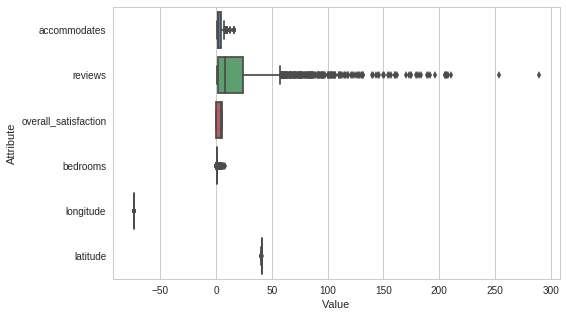
\includegraphics[width = \textwidth]{images/before-std.png}
\caption{Data before standardization}
\label{fig:before-std}
\end{figure}
\par Standardization can be done in many ways, the formula
\[NewValue = (OldValue-Mean)/StandardDeviation\]
is enough for this dataset. The result is shown in the Figure \ref{fig:after-std}
\begin{figure}[h]
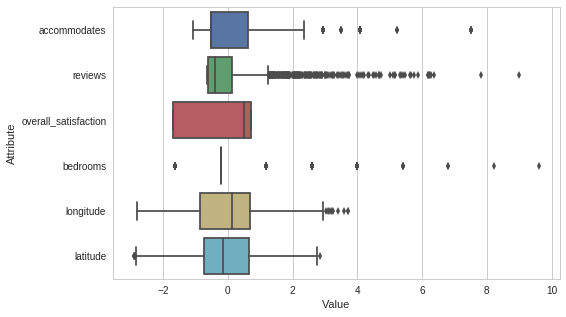
\includegraphics[width = \textwidth]{images/after-std.png}
\caption{Data after standardization}
\label{fig:after-std}
\end{figure}
\section{}

\newpage
\bibliography{biblist}

\end{document}